\section{Ejercicio 7}

%SI QUIEREN AGREGAR IMAGENES COPIEN EL SIGUIENTE CODIGO
%\begin {center}
%\includegraphics[width=12cm]{./graphEj1.jpg}
% grafico.eps: 0x0 pixel, 300dpi, 0.00x0.00 cm, bb=50 50 410 302
%\end {center}

Lote simulado con Round Robin:\\\\
\begin {center}
TaskBatch 17 1\\
TaskBatch 17 2\\
TaskBatch 17 3\\
TaskBatch 17 4\\
TaskBatch 17 5\\
TaskBatch 17 6\\
TaskBatch 17 7\\
\end {center}

\par Diagrama con 2 ciclos de quantum:

\begin {center}
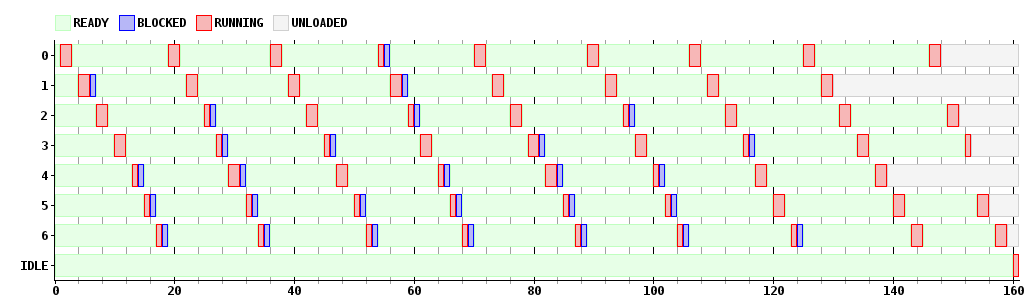
\includegraphics[width=16cm]{../simusched/outputs/ej7/rr-ej7-1-2.png}
\end {center}

\par Diagrama con 5 ciclos de quantum:
\begin {center}
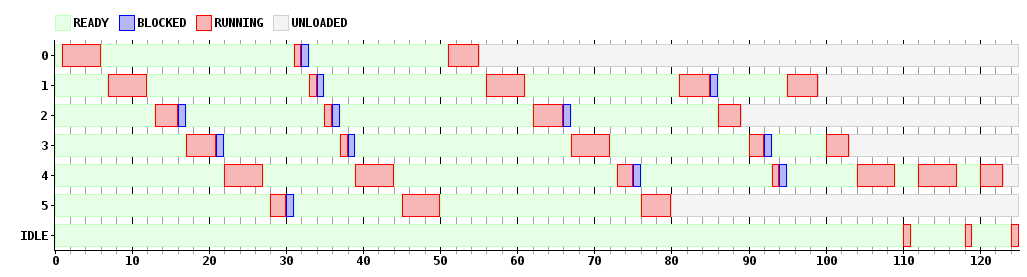
\includegraphics[width=16cm]{../simusched/outputs/ej7/rr-ej7-1-5.png}
\end {center}

\par Diagrama con 7 ciclos de quantum:
\begin {center}
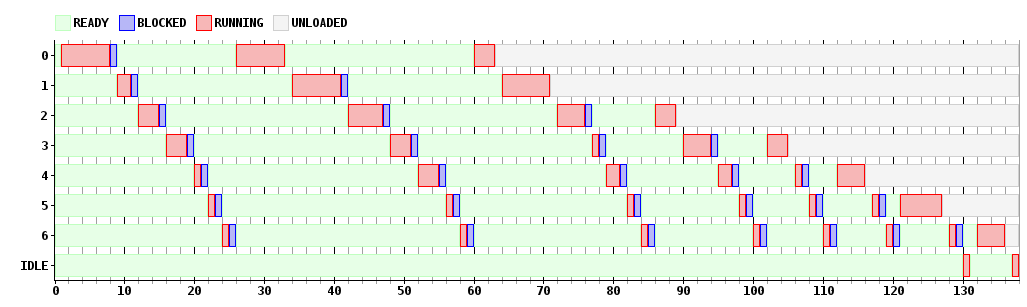
\includegraphics[width=16cm]{../simusched/outputs/ej7/rr-ej7-1-7.png}
\end {center}

\par Diagrama con 9 ciclos de quantum:
\begin {center}
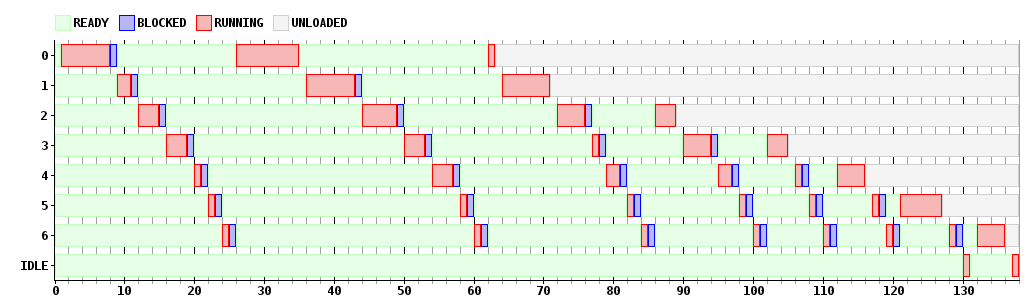
\includegraphics[width=16cm]{../simusched/outputs/ej7/rr-ej7-1-9.png}
\end {center}

\par Diagrama con 12 ciclos de quantum:
\begin {center}
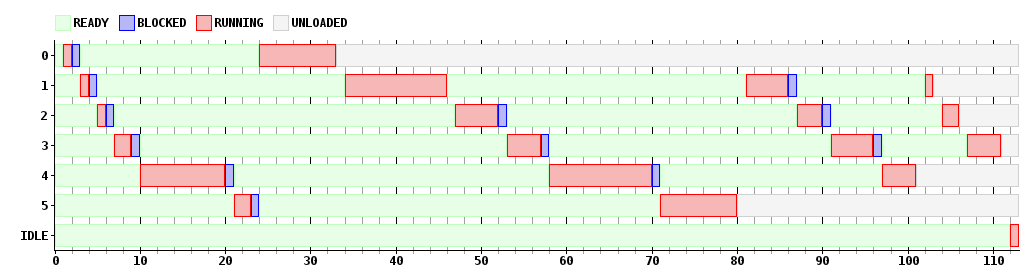
\includegraphics[width=16cm]{../simusched/outputs/ej7/rr-ej7-1-12.png}
\end {center}

\par Diagrama con 15 ciclos de quantum:
\begin {center}
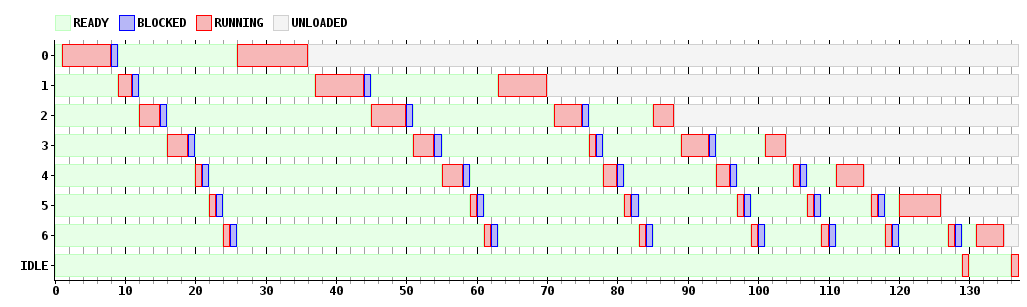
\includegraphics[width=16cm]{../simusched/outputs/ej7/rr-ej7-1-15.png}
\end {center}

\par Diagrama con 21 ciclos de quantum:
\begin {center}
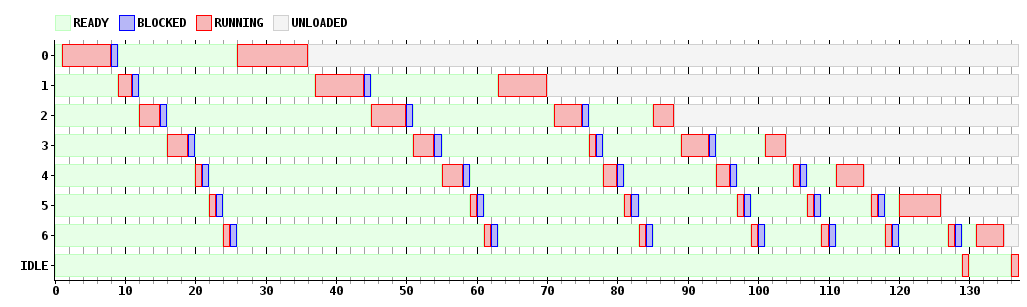
\includegraphics[width=16cm]{../simusched/outputs/ej7/rr-ej7-1-21.png}
\end {center}

Se puede observar que a medida que los ciclos del quantum aumentan, las tareas finalizan más rapido, debido a que se les da más tiempo de ejecución y hay una menor cantidad de cambios de contexto entre los procesos (ahorra el ciclo que tarda en realizarlo). Además, el aumento de quantum incide en el tiempo total de ejecución de un proceso, ya que al ocurrir menos bloqueos, provoca que la tarea finalice más rapido.
\\
Para este lote de tareas en particular, suele ser más eficiente asignarle una cantidad grande de ciclos por quantum,  ya que se realizarán menos bloqueos y menos cambios de contexto, pero no excesiva, porque, como se aprecia en las imágenes, a partir de 12 ciclos por quantum todos tardan lo mismo en finalizar y no mejora la eficiencia, esto es debido a que las tareas se bloquean en menor cantidad y en ningun caso utilizan más del quantum provisto. Por lo tanto, la mejor elección para el quantum es de 12 ciclos.
\\
Con un quantum de 12 ciclos en adelante, se puede notar que lo que más influye en cada proceso son los bloqueos que se producen y no tanto el corte porque no le quedan más ciclos del quantum, produciendo cambios de contexto obligatorios y empeorando bastante el tiempo total de finalización de las tareas, causando un desaprovechamiento de las ventajas del Round Robin frente a otros algoritmos de scheduling, ya que si algo caracteriza a este algoritmo, es de repartir de manera equitativa y racional los recursos, y en este caso se asemeja más a un algoritmo gobernado por bloqueos.


